\documentclass[../main-sheet.tex]{subfiles}
\usepackage{../style}
\graphicspath{ {../img/} }
\backgroundsetup{contents={}}
\begin{document}
\chapter{Epidemic Models and Dynamics of Infectious Diseases}
\section{Epidemiology}
Epidemiology is the study of the distribution and determinants of disease frequency in human population (or in the group of population). It is the cornerstone of public health and informs policy decisions and evidence-based medicine by identifying risk factors for disease and targets for preventive medicine.
\section{Endemic}
Endemic is the habitual presence of a disease within a given geographic area.
\section{Epidemic}
The epidemic is the occurrence in a community or region of a group of illnesses of similar nature in excess of normal expectancy and distributed from a common or propagated source.
\section{Pandemic}
The pandemic is a worldwide epidemic.

There are various types of epidemiological models. We can classify them into two classes:
\begin{enumerate}[label=(\roman*)]
    \item disease with removal,
    \item disease without removal.
\end{enumerate}
\section{Epidemic models with removal}
The model considers the diseases which have the property that individuals once infected by these diseases will be removed from the disease through recovery or death. The individuals removed through recovery are immune temporarily or permanently.

In this case we have three classes of individuals.
\begin{enumerate}[label=(\roman*)]
    \item The susceptible class \((S)\)
    \item The infective class \((I)\)
    \item The removal class \((R)\)
\end{enumerate}
\section{Susceptible class}
The susceptible class consists of those individuals who are not infective but who are capable of catching the disease.
\section{Infective class}
The infective class consists of those individuals who are capable of transmitting the disease to others.
\section{Removal class}
The removal class consists of those individuals who had the disease are dead or recovered or permanently immune or isolated until recovery.
\begin{prob}
    Assume that \(t_0<t_1<t_2\) are equally spaced time values. Let the corresponding population size are \(P_0\), \(P_1\), \(P_2\) respectively. Then the growth rate \(a\) and the carrying capacity \(k\) of logistic population are
    \[
        a=\frac{1}{t_0-t_1}\ln \left[ \frac{\frac{1}{P_2}-\frac{1}{P_1}}{\frac{1}{P_1}-\frac{1}{P_0}} \right]
    \]
    \[
        K=\frac{\frac{2}{P_1}-\frac{1}{P_0}-\frac{1}{P_2}}{\frac{1}{P_1^2}-\frac{1}{P_0P_2}}
    \]
\end{prob}
\begin{soln}
    We have
    \begin{equation}
        P(t)=\frac{K}{1+\left( \frac{K}{P_0}-1 \right)e^{-a(t-t_0)}}
        \label{eq:defnprob1.1}
    \end{equation}
    \begin{align*}
        \Rightarrow\;\frac{1}{P(t)}&=\frac{1}{K}\left[ 1+\left( \frac{K}{P_0}-1 \right)e^{-a(t-t_0)} \right]\\
        &=\frac{1}{K}\left[ 1-e^{-a(t-t_0)} \right]+\frac{1}{P_0}e^{-a(t-t_0)}
    \end{align*}
    \begin{equation}
        \therefore\; \frac{1}{P_1}=\frac{1}{K}\left[ 1-e^{-a(t_1-t_0)} \right]+\frac{1}{P_0}e^{-a(t_1-t_0)}
        \label{eq:defnprob1.2}
    \end{equation}
    and
    \begin{equation}
        \therefore\; \frac{1}{P_2}=\frac{1}{K}\left[ 1-e^{-a(t_2-t_0)} \right]+\frac{1}{P_0}e^{-a(t_2-t_0)}
        \label{eq:defnprob1.3}
    \end{equation}
    Now \eqref{eq:defnprob1.3}-\eqref{eq:defnprob1.2}, we have
    \begin{align*}
        \frac{1}{P_2}-\frac{1}{P_1}&=\frac{1}{K}\left[ 1-e^{-a(t_2-t_0)}-1+e^{-a(t_1-t_0)} \right]+\frac{1}{P_0}e^{-a(t_2-t_0)}-\frac{1}{P_0}e^{-a(t_1-t_0)}\\
        &=\left( \frac{1}{P_1}-\frac{1}{P_0} \right)e^{-a(t_1-t_0)} \quad[\text{Since \(t_0<t_1<t_1\) are equally spaced. So \(t_1=t_2\), \(t_0=t_1\)}]
    \end{align*}
    \begin{equation}
        e^{-a(t_1-t_0)}=\frac{\frac{1}{P_2}-\frac{1}{P_1}}{\left( \frac{1}{P_1}-\frac{1}{P_0} \right)}
        \label{eq:defnprob1.4}
    \end{equation}
    \begin{align*}
        \Rightarrow\;\;& a(t_0-t_1)=\ln\left[ \frac{\frac{1}{P_2}-\frac{1}{P_1}}{\left( \frac{1}{P_1}-\frac{1}{P_0} \right)} \right]\\
        \therefore\;\;& a=\frac{1}{t_0-t_1}\ln\left[ \frac{\frac{1}{P_2}-\frac{1}{P_1}}{\left( \frac{1}{P_1}-\frac{1}{P_0} \right)} \right]
    \end{align*}
    From \eqref{eq:defnprob1.2} we have,
    \begin{align*}
        &\frac{1}{P_1}-\frac{1}{P_0}e^{-a(t_1-t_0)}=\frac{1}{K}\left[ 1-e^{-a(t_1-t_0)} \right]\\
        \Rightarrow\; &K=\frac{ 1-e^{-a(t_1-t_0)}}{\frac{1}{P_1}-\frac{1}{P_0}e^{-a(t_1-t_0)}}\\
        \Rightarrow\; &K=\frac{\displaystyle 1-\frac{\frac{1}{P_2}-\frac{1}{P_1}}{\frac{1}{P_1}-\frac{1}{P_0}} }{\displaystyle \frac{1}{P_1}-\frac{1}{P_0}\left( \frac{\frac{1}{P_2}-\frac{1}{P_1}}{\frac{1}{P_1}-\frac{1}{P_0}} \right)}\qquad [\text{Using \eqref{eq:defnprob1.4}}]\\
        \Rightarrow\; &K=\frac{\displaystyle \frac{\frac{1}{P_1}-\frac{1}{P_0}-\frac{1}{P_2}+\frac{1}{P_1}}{\frac{1}{P_1}-\frac{1}{P_0}}}{\displaystyle \frac{\frac{1}{P_1^2}-\frac{1}{P_0P_1}-\frac{1}{P_0P_2}+\frac{1}{P_0P_1}}{\frac{1}{P_1}-\frac{1}{P_0}}}\\
        \therefore\; &K=\frac{\displaystyle \frac{2}{P_2}-\frac{1}{P_0}+\frac{1}{P_2}}{\displaystyle \frac{1}{P_1^2}-\frac{1}{P_0P_2}}
    \end{align*}
\end{soln}
\begin{prob}
    What do you mean by disease with removal and without removal?
\end{prob}
\begin{soln}
    The epidemic logistic models are various in type such as
    \begin{enumerate}[label=(\roman*)]
        \item Disease without removal
        \item Disease with removal
    \end{enumerate}
    \emph{Disease without removal:} In this case, it is assumed that persons are infected can never be removed from the disease. Therefore, the total population always remains either in \(S\) class or in \(I\) class.

    \emph{Example}: \(SI\) and \(SIS\) models etc. are disease without removal model.\\

    \emph{Disease with removal:} In this model, we consider those diseases which are of the nature, individuals once infected can be removed from the disease through recovery or death. This removal may be temporary or permanent.

    \emph{Example:} Several types of this model are \(SIR\) model, \(SIRS\), \(SEIR\) etc.
\end{soln}
\begin{prob}
    Discuss the \(SI\) model with limiting behavior.
\end{prob}
\begin{soln}
    Without removals, we have\
    \begin{equation}
        S(t)+I(t)=N(t)=\text{ Constant }
        \label{eq:psi1}
    \end{equation}
    where, \(\begin{aligned}[t]
        S(t)&=\text{ The number of susceptible}\\
        I(t)&=\text{ The number of infective person in the population}\\
        N(t)&=\text{ The total population size}
    \end{aligned}\)\\
    Let \(n\) be the initial number of susceptible in the population in which one infected person has been introduced, so that,
    \begin{equation}
        \begin{rcases}
            S(t)+I(t)=n+1\\    
            S(0)=S_0=n\\    
            I(0)=I_0=1    
        \end{rcases}
        \label{eq:psi2}
    \end{equation}
    Due to infection, the number of susceptibles decreases and the number of infected persons increases.\\
    The epidemic model is,
    \begin{align}
        \ddt{S}&=-\beta SI\label{eq:psi3}\\
        \ddt{I}&=\beta SI\label{eq:psi4}
    \end{align}
    From \eqref{eq:psi4},
    \begin{align}
        & \ddt{S}=-\beta SI=-\beta S(n+1-S) \quad\text{ by \eqref{eq:psi2}}\notag\\
        \Rightarrow\;\;& \frac{-1 \D S}{S(n+1-S)}=\beta \D t\notag\\
        \Rightarrow\;\;& -\frac{1 }{n+1}\left( \frac{1}{S}+\frac{1}{n+1-S} \right)=\beta \D t\notag\\
        \Rightarrow\;\;& -\int \frac{1 }{S}\D S-\int \frac{1}{n+1-S} \D S=\int(n+1)\beta \D t\notag\\
        \Rightarrow\;\;& -\ln{S}+\ln({n+1-S})=(n+1)\beta t+\ln c\quad\text{ where \(c\) is a constant}\label{eq:psi5}
    \end{align}
    By using the initial conditions \eqref{eq:psi2}, we have
    \begin{align}
        & -\ln{S_0}+\ln({n+1-S_0})=(n+1)\beta\cdot0+\ln c\notag\\
        \Rightarrow\;\;& -\ln n+\ln({n+1-n})=\ln c\notag\\
        \Rightarrow\;\;& -\ln n=\ln c\notag\\
        \intertext{Putting the value of \(ln c\) in \eqref{eq:psi5} we get,}
        \Rightarrow\;\;& -\ln{S}+\ln({n+1-S})=(n+1)\beta t-\ln n\notag\\
        \Rightarrow\;\;& \ln\frac{n(n+1-S)}{S}=(n+1)\beta t\notag\\
        \Rightarrow\;\;& \frac{n(n+1-S)}{S}=e^{(n+1)\beta t}\notag\\
        \Rightarrow\;\;& {n(n+1)-nS}=Se^{(n+1)\beta t}\notag\\
        \Rightarrow\;\;& {n(n+1)}=nS+Se^{(n+1)\beta t}\notag\\
        \Rightarrow\;\;& S=S(t)=\frac{n(n+1)}{n+e^{(n+1)\beta t}}\label{eq:psi6}
    \end{align}
    From \eqref{eq:psi4}, we have
    \begin{align}
        &\ddt{I}=\beta SI=\beta I(n+1-I)\quad \text{ [by \eqref{eq:psi2}]}\notag\\
        \Rightarrow\;\;&\frac{\D I}{I(n+1-I)}=\beta \D t\notag\\
        \Rightarrow\;\;&\int\frac{1}{n+1}\left( \frac{1}{I}+\frac{1}{n+1-I} \right)\D I=\int \beta \D t\notag\\
        \Rightarrow\;\;&\int\left( \frac{1}{I}+\frac{1}{n+1-I} \right)\D I=\int(n+1) \beta \D t\notag\\
        \Rightarrow\;\;&\ln {I}-\ln ({n+1-I}) =(n+1) \beta t+\ln A\label{eq:psi7}\quad\text{ where \(\ln A\) is a constant}
    \end{align}
    Initially, \(t=0\), \(I_0=1\), so we get,
    \begin{align*}
        &\ln {I_0}-\ln ({n+1-I_0}) =(n+1) \beta \cdot 0+\ln A\\
        \Rightarrow\;\;&\ln 1-\ln ({n+1-1}) =0+\ln A\\
        \Rightarrow\;\;&-\ln n =\ln A\\
        \Rightarrow\;\;&\ln A =-\ln n
    \end{align*}
    Putting this value in \eqref{eq:psi7}, we get.
    \begin{align}
        &\ln {I}-\ln ({n+1-I}) =(n+1) \beta t-\ln n\notag\\
        \Rightarrow\;\;&\ln \frac{nI}{n+1-I}=(n+1) \beta t\notag\\
        \Rightarrow\;\;&\frac{nI}{n+1-I}=e^{(n+1) \beta t}\notag\\
        \Rightarrow\;\;&{nI}=(n+1)e^{(n+1) \beta t}-Ie^{(n+1) \beta t}\notag\\
        \Rightarrow\;\;&\left[ n+e^{(n+1) \beta t} \right]I=(n+1)e^{(n+1) \beta t}\notag\\
        \Rightarrow\;\;&I=\frac{(n+1)e^{(n+1) \beta t}}{n+e^{(n+1) \beta t} }\label{eq:psi8}
    \end{align}
    From \eqref{eq:psi6} and \eqref{eq:psi8}, we have,
    \[
        \lim_{t\to \infty}S(t)=\frac{n(n+1)}{n+e^\infty}=\frac{n(n+1)}{\infty}=0
    \]
    and
    \begin{align*}
        \lim_{t\to \infty}I(t)&=\lim_{t\to \infty}\frac{(n+1)e^{(n+1) \beta t}}{n+e^{(n+1) \beta t} }\\
        &=\lim_{t\to \infty}\frac{(n+1)}{ne^{-(n+1) \beta t} +1}\\
        &=\frac{(n+1)}{ne^{-\infty} +1}\\
        &=n+1
    \end{align*}
    Thus, ultimately all persons will be infected.
\end{soln}
\begin{prob}
    Consider the epidemic model
    \begin{align*}
        S'&=-\alpha SI\\
        I'&=\alpha SI-\gamma I\\
        R'&=\gamma I
    \end{align*}
    Interpret the state variables \(S(t)\), \(I(t)\), \(R(t)\) and the model parameters.\\
    Find the co-ordinate on which the infection (disease) will ultimately die out.
\end{prob}
\begin{soln}
    Let,
    \begin{align*}
        S(t)&=\text{ The number of susceptibles who can catch the disease.}\\
        I(t)&=\text{ The number of infected persons in the population.}\\
        R(t)&=\text{ The number of those removed from the population by recovery, death or by any other means.}\\
        N(t)&=\text{ The total number of population size.}
    \end{align*}
    The progress of individuals is schematically represented by \(S\to I\to R\). Such models are often called \(SIR\) models.\\
    Here we assume that
    \begin{enumerate}[label=(\roman*)]
        \item The gain in the infective class is at a rate proportional to the number of infectives and susceptibles, that is \(\alpha SI\), where \(\alpha>0\) is a constant parameter.
        \item The rate of removed of infectives to the removal class is proportional to the number of infectives, that is \(\gamma I\) where \(\gamma >0\) is a constant.
        \item The incuration period is short enough to be negligible.
    \end{enumerate}
    The model based on the above assumption is,
    \begin{align}
        \ddt{S}&=-\alpha SI\label{eq:psir1}\\
        \ddt{I}&=\alpha SI-\gamma I\label{eq:psir2}\\
        \ddt{R}&=\gamma I\label{eq:psir3}
    \end{align}
    where, \(\alpha>0\) is the infection rate and \(\gamma>0\) is the removal rate of infectives.\\
    The above model has initial conditions
    \begin{equation}
        S(0)=S_0>0,\qquad I(0)=I_0>0,\qquad R(0)=0\label{eq:psir4}
    \end{equation}
    From \eqref{eq:psir2}, we write,
    \[
        \left[ \ddt{I} \right]_{t=0}=I_0 (\alpha S_0-\gamma)\;\;\begin{cases}
            >0& \text{ if } S_0>\frac{\gamma}{\alpha}\\
            <0& \text{ if } S_0<\frac{\gamma}{\alpha}
        \end{cases}
    \]
    where \(\frac{\gamma}{\alpha}\) is relative removal rate.\\
    Since from \eqref{eq:psir1} we have, \(\ddt{S}\leq 0,\quad S\leq S_0\).\\
    If \(S_0<\frac{\gamma}{\alpha}\), then
    \begin{equation}
        \ddt{I}=I(\alpha S-\gamma)\leq 0 \label{eq:psir5}
    \end{equation}
    for all \(t>0\) in which case \(I_0>I\to 0\) as \(t\to \infty\) and so the infection dies out that is no epidemic can occur.

    On the other hand, if \(S_0>\frac{\gamma}{\alpha}\) then \(I(t)\) initially increases and we have an epidemic. The term epidemic means that, \(I(t)>I_0\) for some \(t>0\).\\
    Again from \eqref{eq:psir1} and \eqref{eq:psir2}, we have
    \begin{align}
        &\frac{\D I}{\D S}=\frac{\alpha SI-\gamma I}{-\alpha SI}=-1+\frac{\gamma}{\alpha S}\notag\\
        \Rightarrow\;\;&\int \D I=-\int \D S+ \rho\int\frac{1}{S}\D S,\quad\text{where }\rho=\frac{\gamma}{\alpha}\notag\\
        \Rightarrow\;\;&\int \D I=-\int \D S+ \rho\int\frac{1}{S}\D S,\quad\text{where }\rho=\frac{\gamma}{\alpha}\notag\\
        \Rightarrow\;\;&I=-S+ \rho\ln{S}+\text{ constant }\notag\\
        \Rightarrow\;\;&I+S- \rho\ln{S}=\text{ constant }=I_0+S_0- \rho\ln{S_0}\label{eq:psir6}
    \end{align}
    Here \(R(0)=0\), so \(0\leq S+I< N\)\\
    From \eqref{eq:psir5}, \(I\) will be maximized if 
    \begin{align*}
        &\ddt{I}=0\\
        \Rightarrow\;\;&I(\alpha S-\gamma)=0\\
        \Rightarrow\;\;&S=\frac{\gamma}{\alpha}=\rho \qquad \text{since, }I\neq0
    \end{align*}
    Putting, \(S=\rho\) in \eqref{eq:psir6} we get,
    \begin{align}
        &I_{\max} +\rho-\rho \ln \rho=I_0+S_0-\rho \ln S_0\notag\\
        \Rightarrow\;\; &I_{\max} =\rho \ln \rho-\rho+I_0+S_0-\rho \ln S_0\notag\\
        \Rightarrow\;\; &I_{\max} =(I_0-S_0)-\rho +\rho \ln \left( \frac{\rho}{S_0} \right)\label{eq:psir7}\\
        \Rightarrow\;\; &I_{\max} =N-\rho +\rho \ln \left( \frac{\rho}{S_0} \right),\qquad N=I_0+S_0\notag
    \end{align}
    If \(I_0>0\), and \(S_0>\rho\), then the phase trajectory start with \(S>\rho\), also in this case \(I\) increases from \(I_0\) and hence an epidemic ensure.

    If \(S_0<\rho\) then \(I\) decreases from \(I_0\) and as such no epidemic occurs.
\end{soln}
\begin{prob}
    Describe the \(SIR\) model for an epidemic. Discuss the asymptotic behavior of \(S(t)\), \(I(t)\), \(R(t)\).\\
    or,\\
    Describe the deterministic epidemic model with removal. Find the condition on which the infection die out or spread throughout the population.\\
    or,\\
    Discuss the Kermack-Mckendric epidemic model. Analyze the asymptotic behavior of the solution of the model.
\end{prob}
\begin{soln}
    The \(SIR\) model is given by,
    \begin{align}
        \ddt{S}&=S'=-\alpha SI\label{eq:psir2.1}\\
        \ddt{I}&=I'=\alpha SI-\gamma I\label{eq:psir2.2}\\
        \ddt{R}&=R'=\gamma I\label{eq:psir2.3}
    \end{align}
    Here,
    \begin{align*}
        S(t)&=\text{ The number of susceptibles who can catch the disease.}\\
        I(t)&=\text{ The number of infected persons in the population.}\\
        R(t)&=\text{ The number of those removed from the population by recovery, death or by any other means.}\\
        \alpha&=\text{ The infection rate which is positive.}\\
        \gamma&=\text{ The removal rate of infective which is positive.}\\
        \rho=\frac{\gamma}{\alpha}&=\text{ It is a pure number which is the ratio of removal rate of infectives with infection rate.}
    \end{align*}
    The above model has initial conditions
    \begin{equation}
        S(0)=S_0>0,\qquad I(0)=I_0>0,\qquad R(0)=0\label{eq:psir2.4}
    \end{equation}
    From \eqref{eq:psir2}, we write,
    \[
        \left[ \ddt{I} \right]_{t=0}=I_0 (\alpha S_0-\gamma)\;\;\begin{cases}
            >0& \text{ if } S_0>\rho=\frac{\gamma}{\alpha}\\
            <0& \text{ if } S_0<\rho=\frac{\gamma}{\alpha}
        \end{cases}
    \]
    Since from \eqref{eq:psir2.1} we have
    \[
        \ddt{s}\leq 0,\quad S\leq S_0
    \]
    If \(S_0<\frac{\gamma}{\alpha}\), then \(\ddt{I}=I(\alpha S-\gamma)\leq 0 \)
    for all \(t>0\) in which case \(I_0>I(t)\to 0\) as \(t\to \infty\). So the infection (disease) ultimately die out.

    From \eqref{eq:psir2.1}, \(S(t)\) is monotonic decreasing function of \(t\). So that \(S(t)\leq S_0\).

    This shows that \(S(t)\) is bounded below \((S(t)\leq 0)\), we find that \(\lim_{t\to \infty}S(t)=S(\infty)\) exist.

    From \eqref{eq:psir2.3}, we have \(R(t)\) is a monotonic increasing function of \(t\) and is bounded above \(R(t)\leq N\), we see that \(\lim_{t\to \infty}R(t)=R(\infty)\) exist.

    Again, since \(S(t)+I(t)+R(t)=N\) for all \(t\).\\
    We find that \(\lim_{t\to \infty}I(t)=I(\infty)\) also exist.
\end{soln}
\begin{prob}
    Describe \(SIS\) model.
\end{prob}
\begin{soln}
    The \(SIS\) model is given by
    \begin{align}
        \ddt{S}&=-\alpha SI-\beta I \label{eq:si1}\\
        \ddt{I}&=\alpha SI-\beta I \label{eq:si2}
    \end{align}
    where, \(\begin{aligned}[t]
        S(t)&= \text{ the number of susceptible individuals at time } t\\
        I(t)&= \text{ the number of infected individuals at time } t
    \end{aligned}\)\\
    where \(\alpha\) and \(\beta\) are the constant and
    \begin{equation}
        S+I=N\label{eq:si3}
    \end{equation}
    where \(N\) is the size of the population.\\

    In this model we assume that a susceptible person becomes infected at a rate proportional to \(SI\) and then an infected person recovers and again becomes susceptible at rate proportional to \(I_0\).\\
    The above model has the initial condition, \(S(0)=S_0\), \(I(0)=I_0\) at \(t=0\).\\
    We have, \(S(t)+I(t)=S_0+I_0=\) constant \(=N\).\\
    From \eqref{eq:si2},
    \begin{align}
        &\ddt{I}=\alpha (N-I)I-\beta I\notag\\
        \Rightarrow\;&\ddt{I}=\alpha NI-\alpha I^2-\beta I\notag\\
        \Rightarrow\;&\ddt{I}=I(\alpha N-\beta)-\alpha I^2\notag\\
        \Rightarrow\;&\ddt{I}=K I-\alpha I^2\qquad \text{where, }K=\alpha N-\beta\notag\\
        \Rightarrow\;&\ddt{I}=KI\left( 1-\frac{\alpha}{K}I \right)\notag\\
        \Rightarrow\;&\frac{\D I}{I\left( 1-\frac{\alpha}{K}I \right)}=K\D t\notag\\
        \Rightarrow\;&\left[ \frac{1}{I}+\frac{1}{\frac{K}{\alpha}-I} \right]\D I=K\D t\notag\\
        \Rightarrow\;&\ln{I}+\ln\left[\frac{K}{\alpha}-I \right]=Kt+\ln A\notag\\
        \Rightarrow\;& \ln \frac{I}{A\left[ \frac{K}{\alpha}-I \right]}=Kt\notag\\
        \Rightarrow\;& \frac{I}{A\left[ \frac{K}{\alpha}-I \right]}=e^{Kt}\notag\\
        \Rightarrow\;& A=\frac{I}{\left[ \frac{K}{\alpha}-I \right]e^{Kt}}\label{eq:si4}\\
        \Rightarrow\;& A\frac{K}{\alpha}e^{Kt}-AIe^{kt}=I\notag\\
        \Rightarrow\;& I=\frac{A\frac{K}{\alpha}e^{Kt}}{1+Ae^{Kt}}\label{eq:si5}
    \end{align}
    Initially, \(t=0\), \(I=I_0\), \(A=\frac{I_0}{\frac{k}{\alpha}-I_0}\)\\
    From \eqref{eq:si5},
    \begin{align*}
        I&=\frac{I_0 \left[\frac{K}{\alpha}\right]e^{Kt}}{\left(\frac{k}{\alpha}-I_0\right) \left[1+\frac{I_0}{\frac{k}{\alpha}-I_0}\right]e^{Kt}}\\
        &=\frac{I_0 \frac{K}{\alpha}e^{Kt}}{\frac{k}{\alpha}-I_0+{I_0}e^{Kt}}\\
        &=\frac{\frac{K}{\alpha}I_0 e^{kt}}{I_0\frac{k}{\alpha}\left[ \frac{1}{I_0}+\left( e^{kt}-1 \right)\frac{\alpha}{k} \right]}\\
        &=\frac{e^{kt}}{\frac{\alpha}{k}\left( e^{kt}-1 \right)+\frac{1}{I_0}}\qquad \text{where }k\neq0
    \end{align*}
    When \(k=0\), 
    \begin{align*}
        &\ddt{I}=-\alpha I^2\\
        \Rightarrow\;&-\frac{\D I}{I^2}=\alpha \D t\\
        \Rightarrow\;&\frac{1}{I}=\alpha +B\\
        \intertext{Initially, \(t=0\), \(I=I_0\)}
        \therefore\;&B=\frac{1}{I_0}\\
        \therefore\;&\frac{1}{I}=\alpha +\frac{1}{I_0}\\
        \Rightarrow\;&I=\frac{1}{\alpha t+\frac{1}{I_0}}
    \end{align*}
    \[
        I(t)=\begin{cases}
        \frac{e^{kt}}{\frac{\alpha}{k}\left( e^{kt}-1 \right)+\frac{1}{I_0}},&k\neq 0\\
        \frac{1}{\alpha t+\frac{1}{I_0}},&k=0
        \end{cases}
    \]
    Since, \(S(t)+I(t)=N\), i.e., \(S(t)=N-I(t)\)\\
    We get,
    \[
        S(t)=\begin{cases}
        N-\frac{e^{kt}}{\frac{\alpha}{k}\left( e^{kt}-1 \right)+\frac{1}{I_0}},&k\neq 0\\
        N-\frac{1}{\alpha t+\frac{1}{I_0}},&k=0
        \end{cases}
    \]
    We have, \(k=\alpha N-\beta\quad\Rightarrow\;\frac{K}{\alpha}=N-\frac{\beta}{\alpha}=N-\rho\) where \(\rho=\frac{\beta}{\alpha}\) is known relative removal rate.\\
    Now, as \(\begin{aligned}[t]
        t&\to \infty,\\
        I(t)&\to \frac{k}{\alpha}=N-\rho\quad \text{if }k>0, \text{i.e., }N>\rho\\
        \text{and }I(t)&\to 0\quad \text{if }k\leq 0, \text{i.e., }N\leq\rho
    \end{aligned}\)\\

    These results are shown in the diagram.
    \begin{center}
        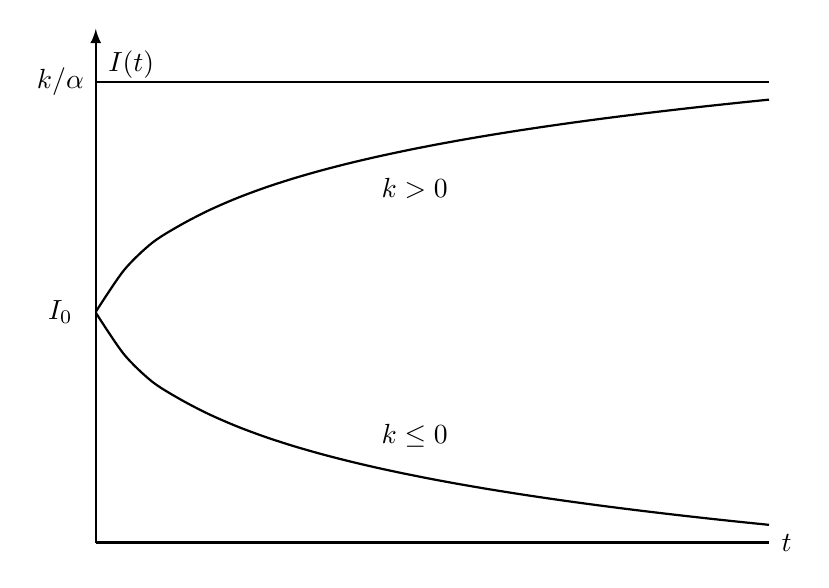
\begin{tikzpicture}[scale=.9]
            \draw[thick] (0.5,3.25)--(10,3.25);
            \draw[thick] (0.5,-3.25)--(10,-3.25);
            \draw[thick,-latex] (0.5,-3.25)--(.5,4);
            \draw [thick, smooth, domain=0.5:10] plot ({\x}, {ln(.1*\x)+3});
            \draw [thick, smooth, domain=0.5:10] plot ({\x}, {-(ln(.1*\x)+3)});
            
            \node at (10.25,-3.25) {$t$};
            \node at (0,0) {$I_0$};
            \node at (0,3.25) {$k/\alpha$};
            \node at (1,3.5) {$I(t)$};
            \node at (5,1.75) {$k>0$};
            \node at (5,-1.75) {$k\leq 0$};
            \end{tikzpicture}
    \end{center}
\end{soln}
\end{document}